\chapter{Perancangan dan Relasi Antar Tabel}

\section{Perancangan dan Relasi Antar Tabel}
Pada bagian ini kita membuat perancangan dan relasinya yang sudah kita buat sebagai berikut : 
\begin{figure}[H]
	\centering
	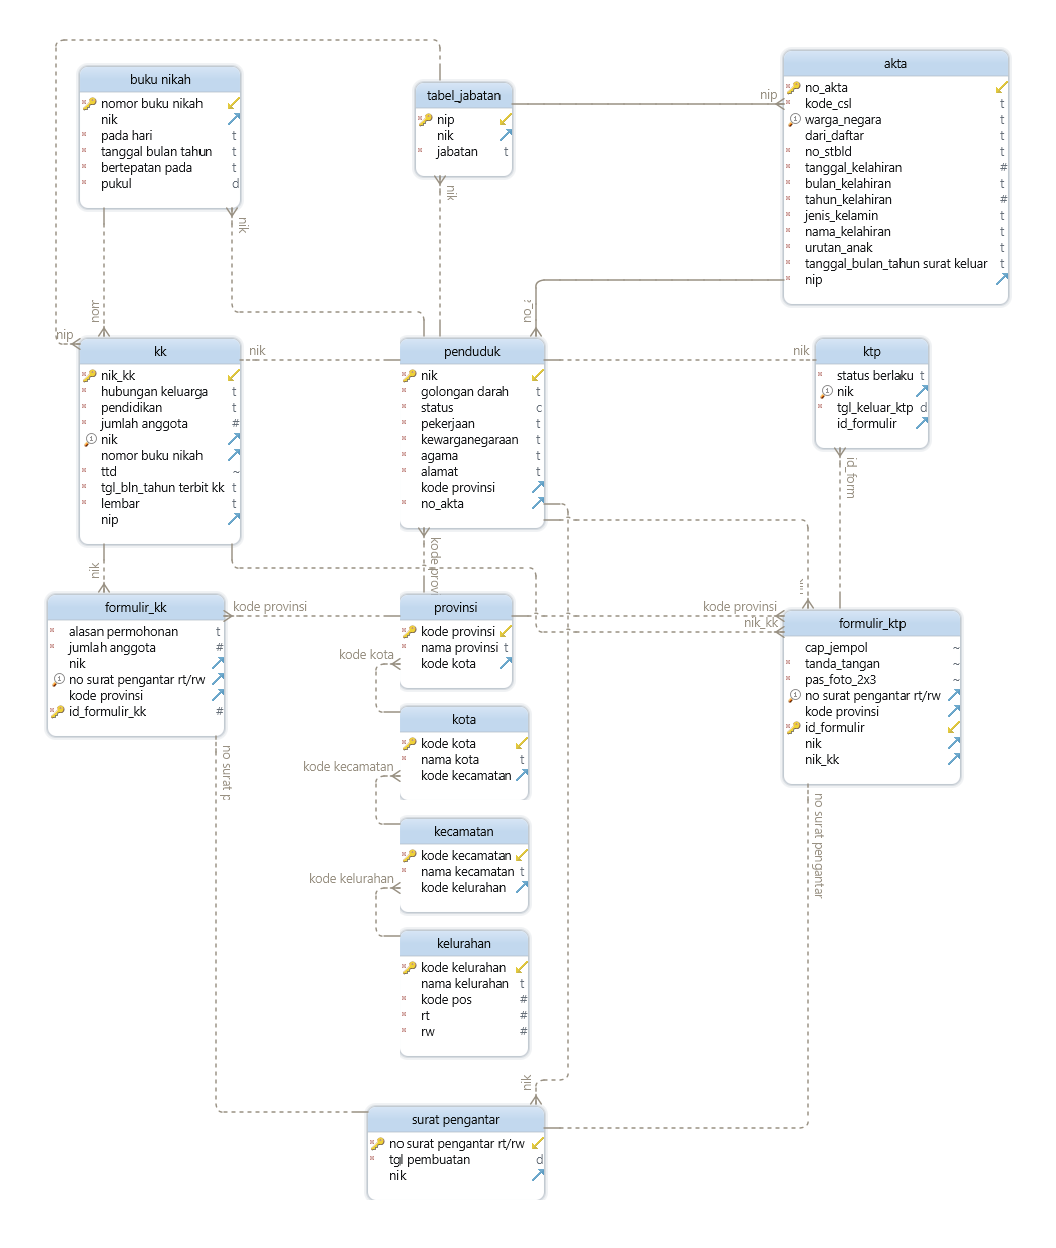
\includegraphics[width=12cm]{figures/0002.png}
	\caption{Tabel Database Perancangan dan Relasi Tabel.}
\end{figure}
Hasil foreign key dari tabel yang memiliki primary key ketika direlasikan juga sudah terlihat dan ini hasil dari beberapa tabel yang sudah berelasi :
\begin{figure}[H]
	\centering
	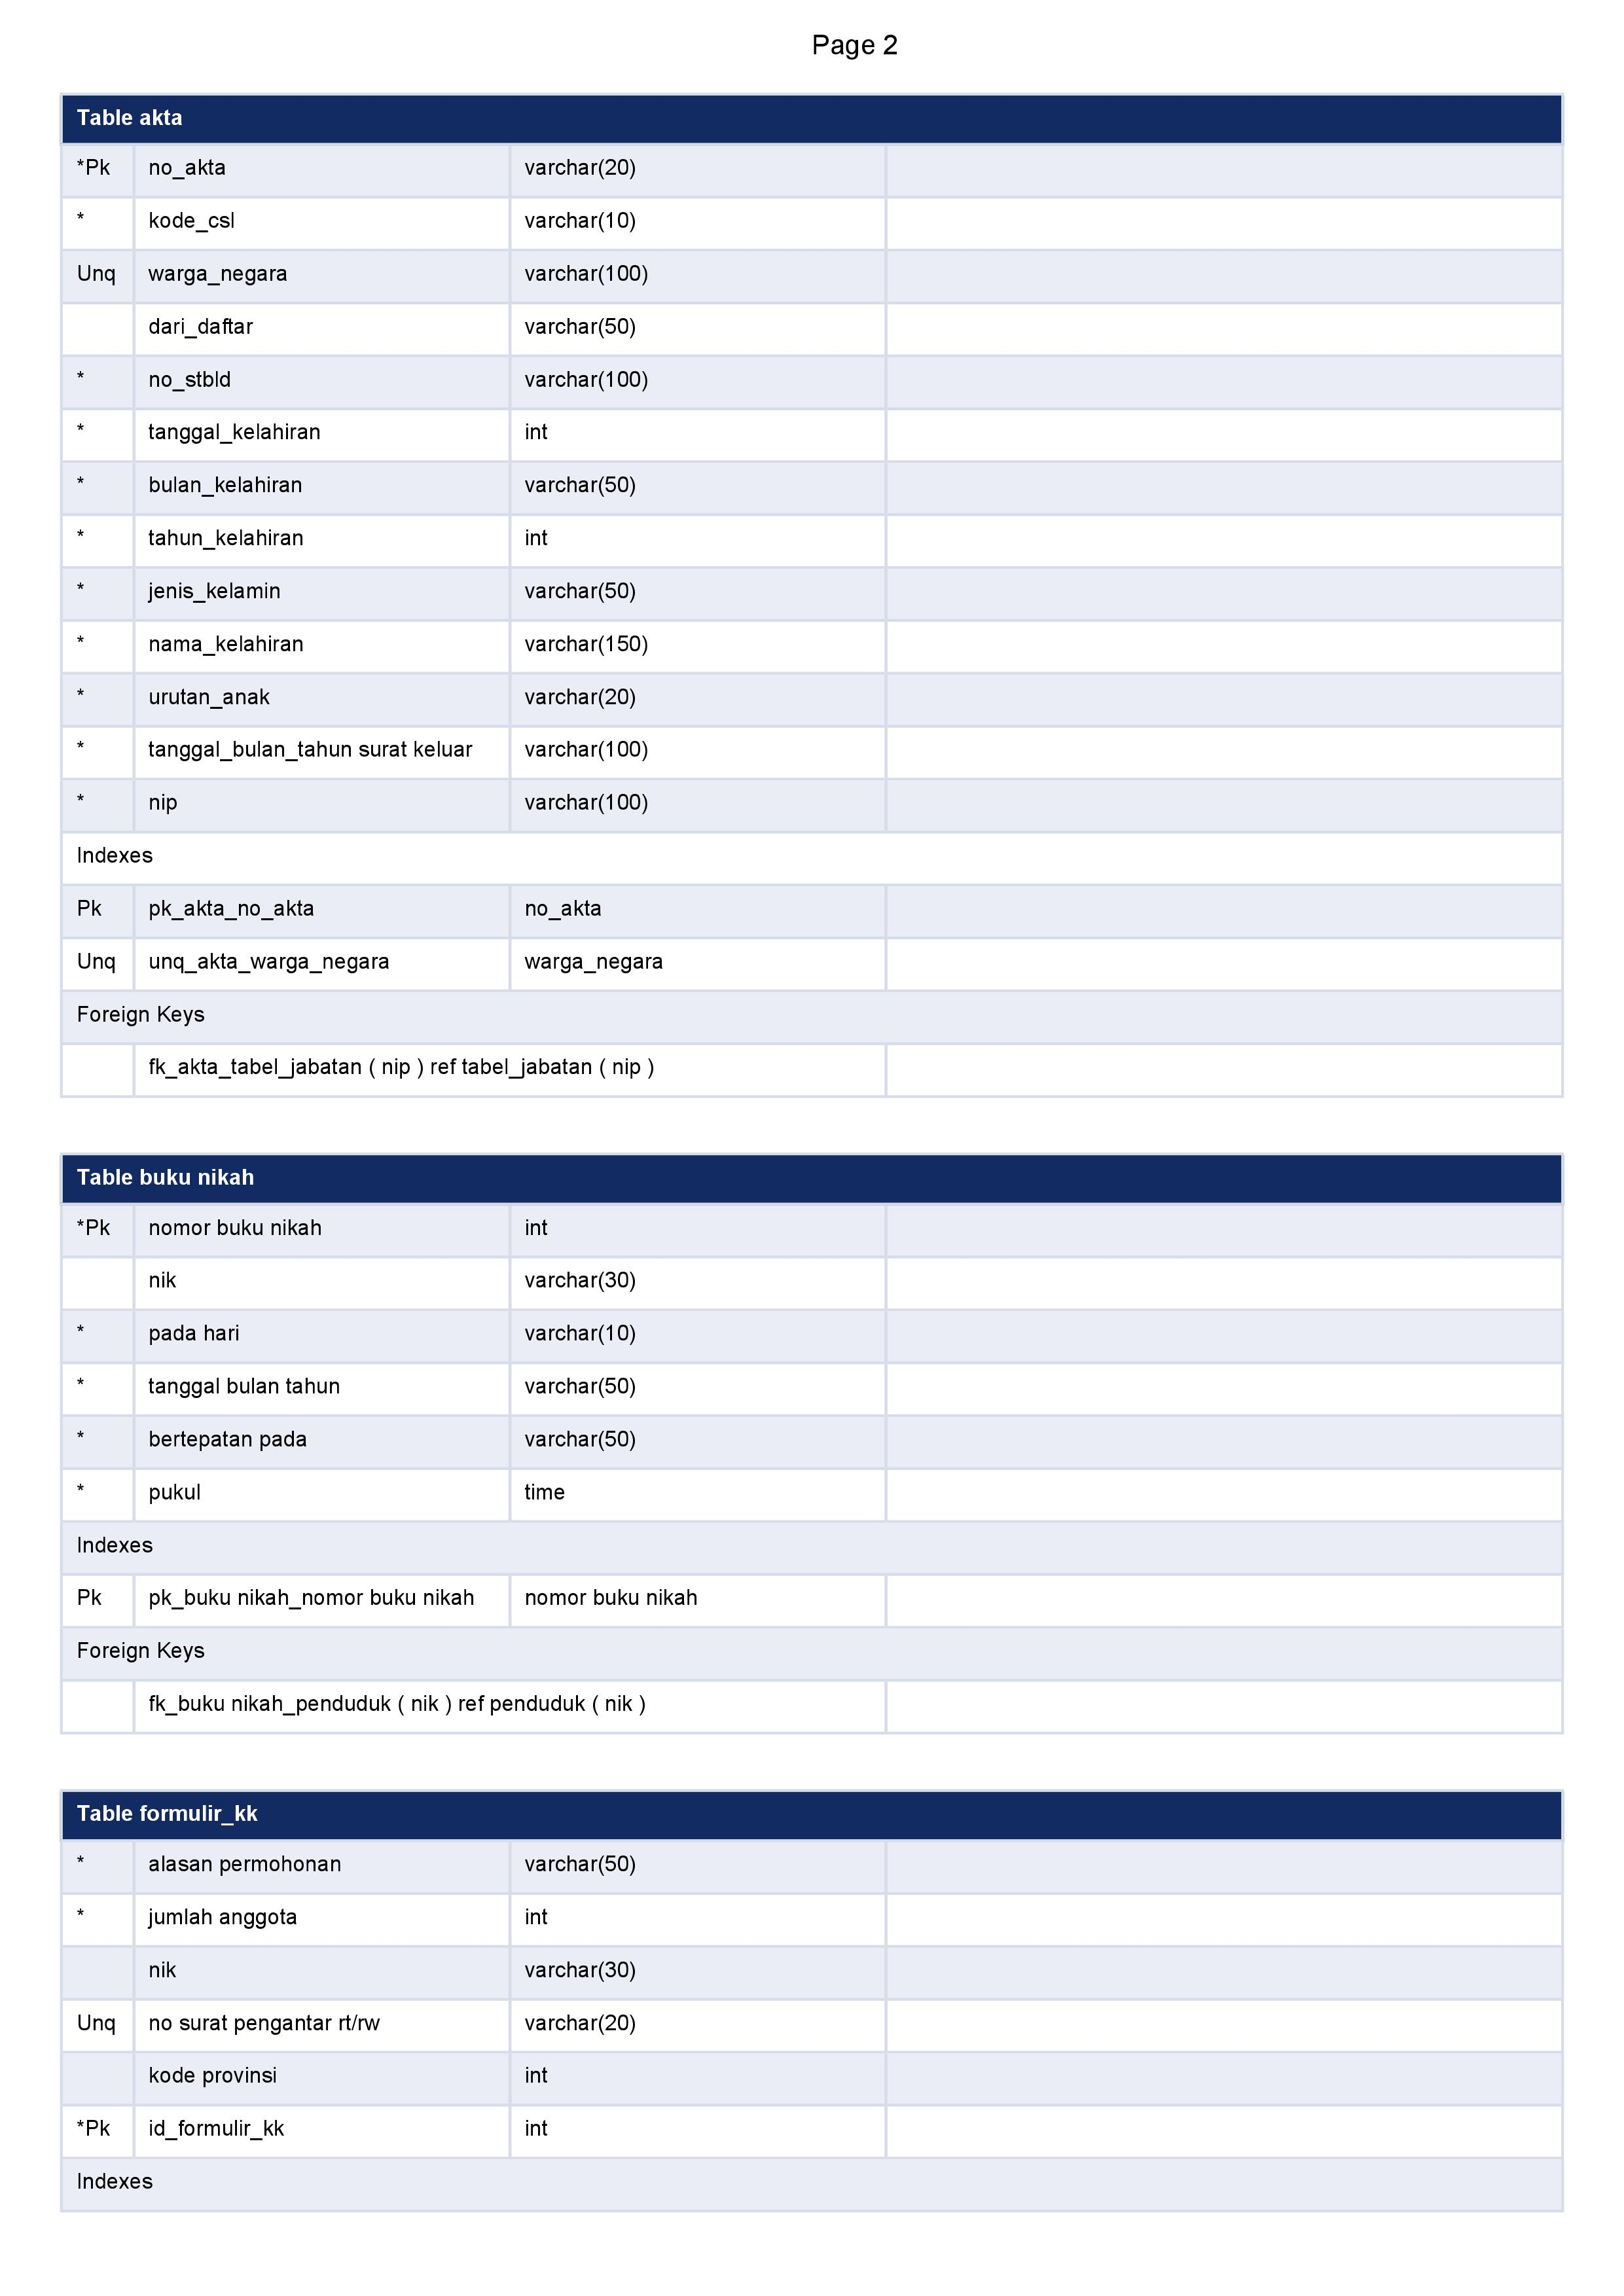
\includegraphics[width=12cm]{figures/0003.jpg}
	\caption{Relasi 1}
\end{figure}
\begin{figure}[H]
	\centering
	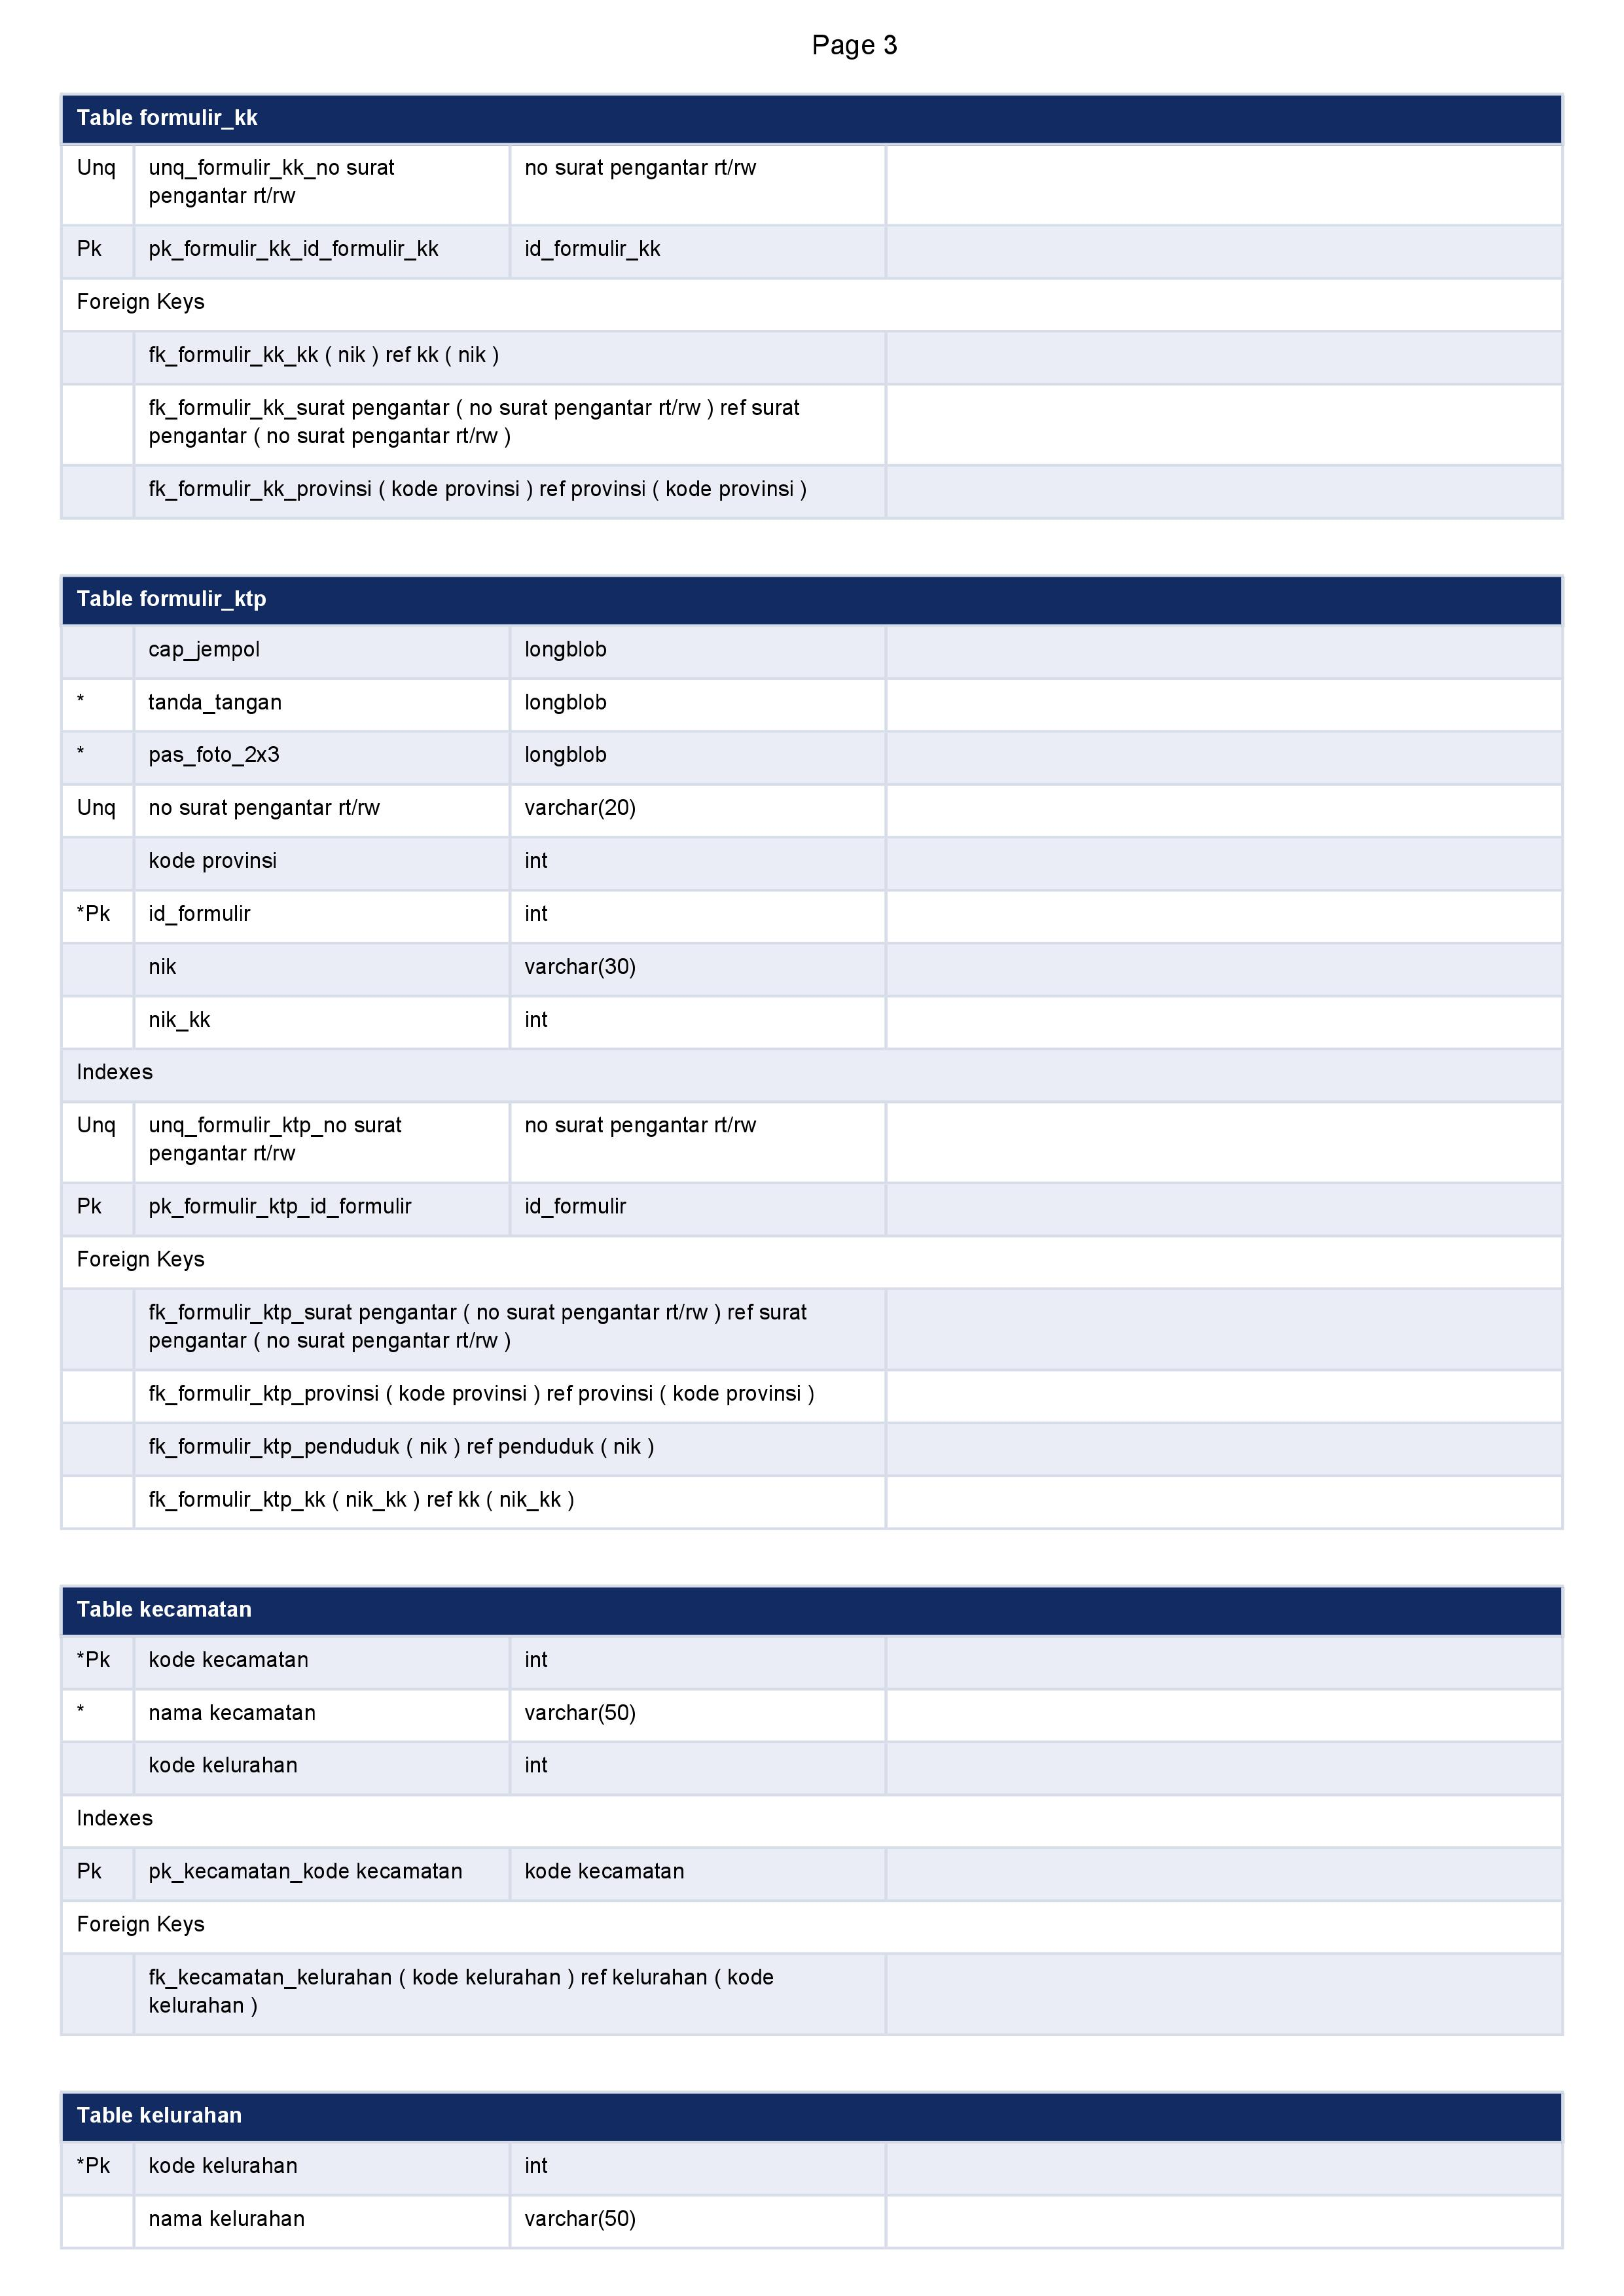
\includegraphics[width=12cm]{figures/0004.jpg}
	\caption{Relasi 2}
\end{figure}
\begin{figure}[H]
	\centering
	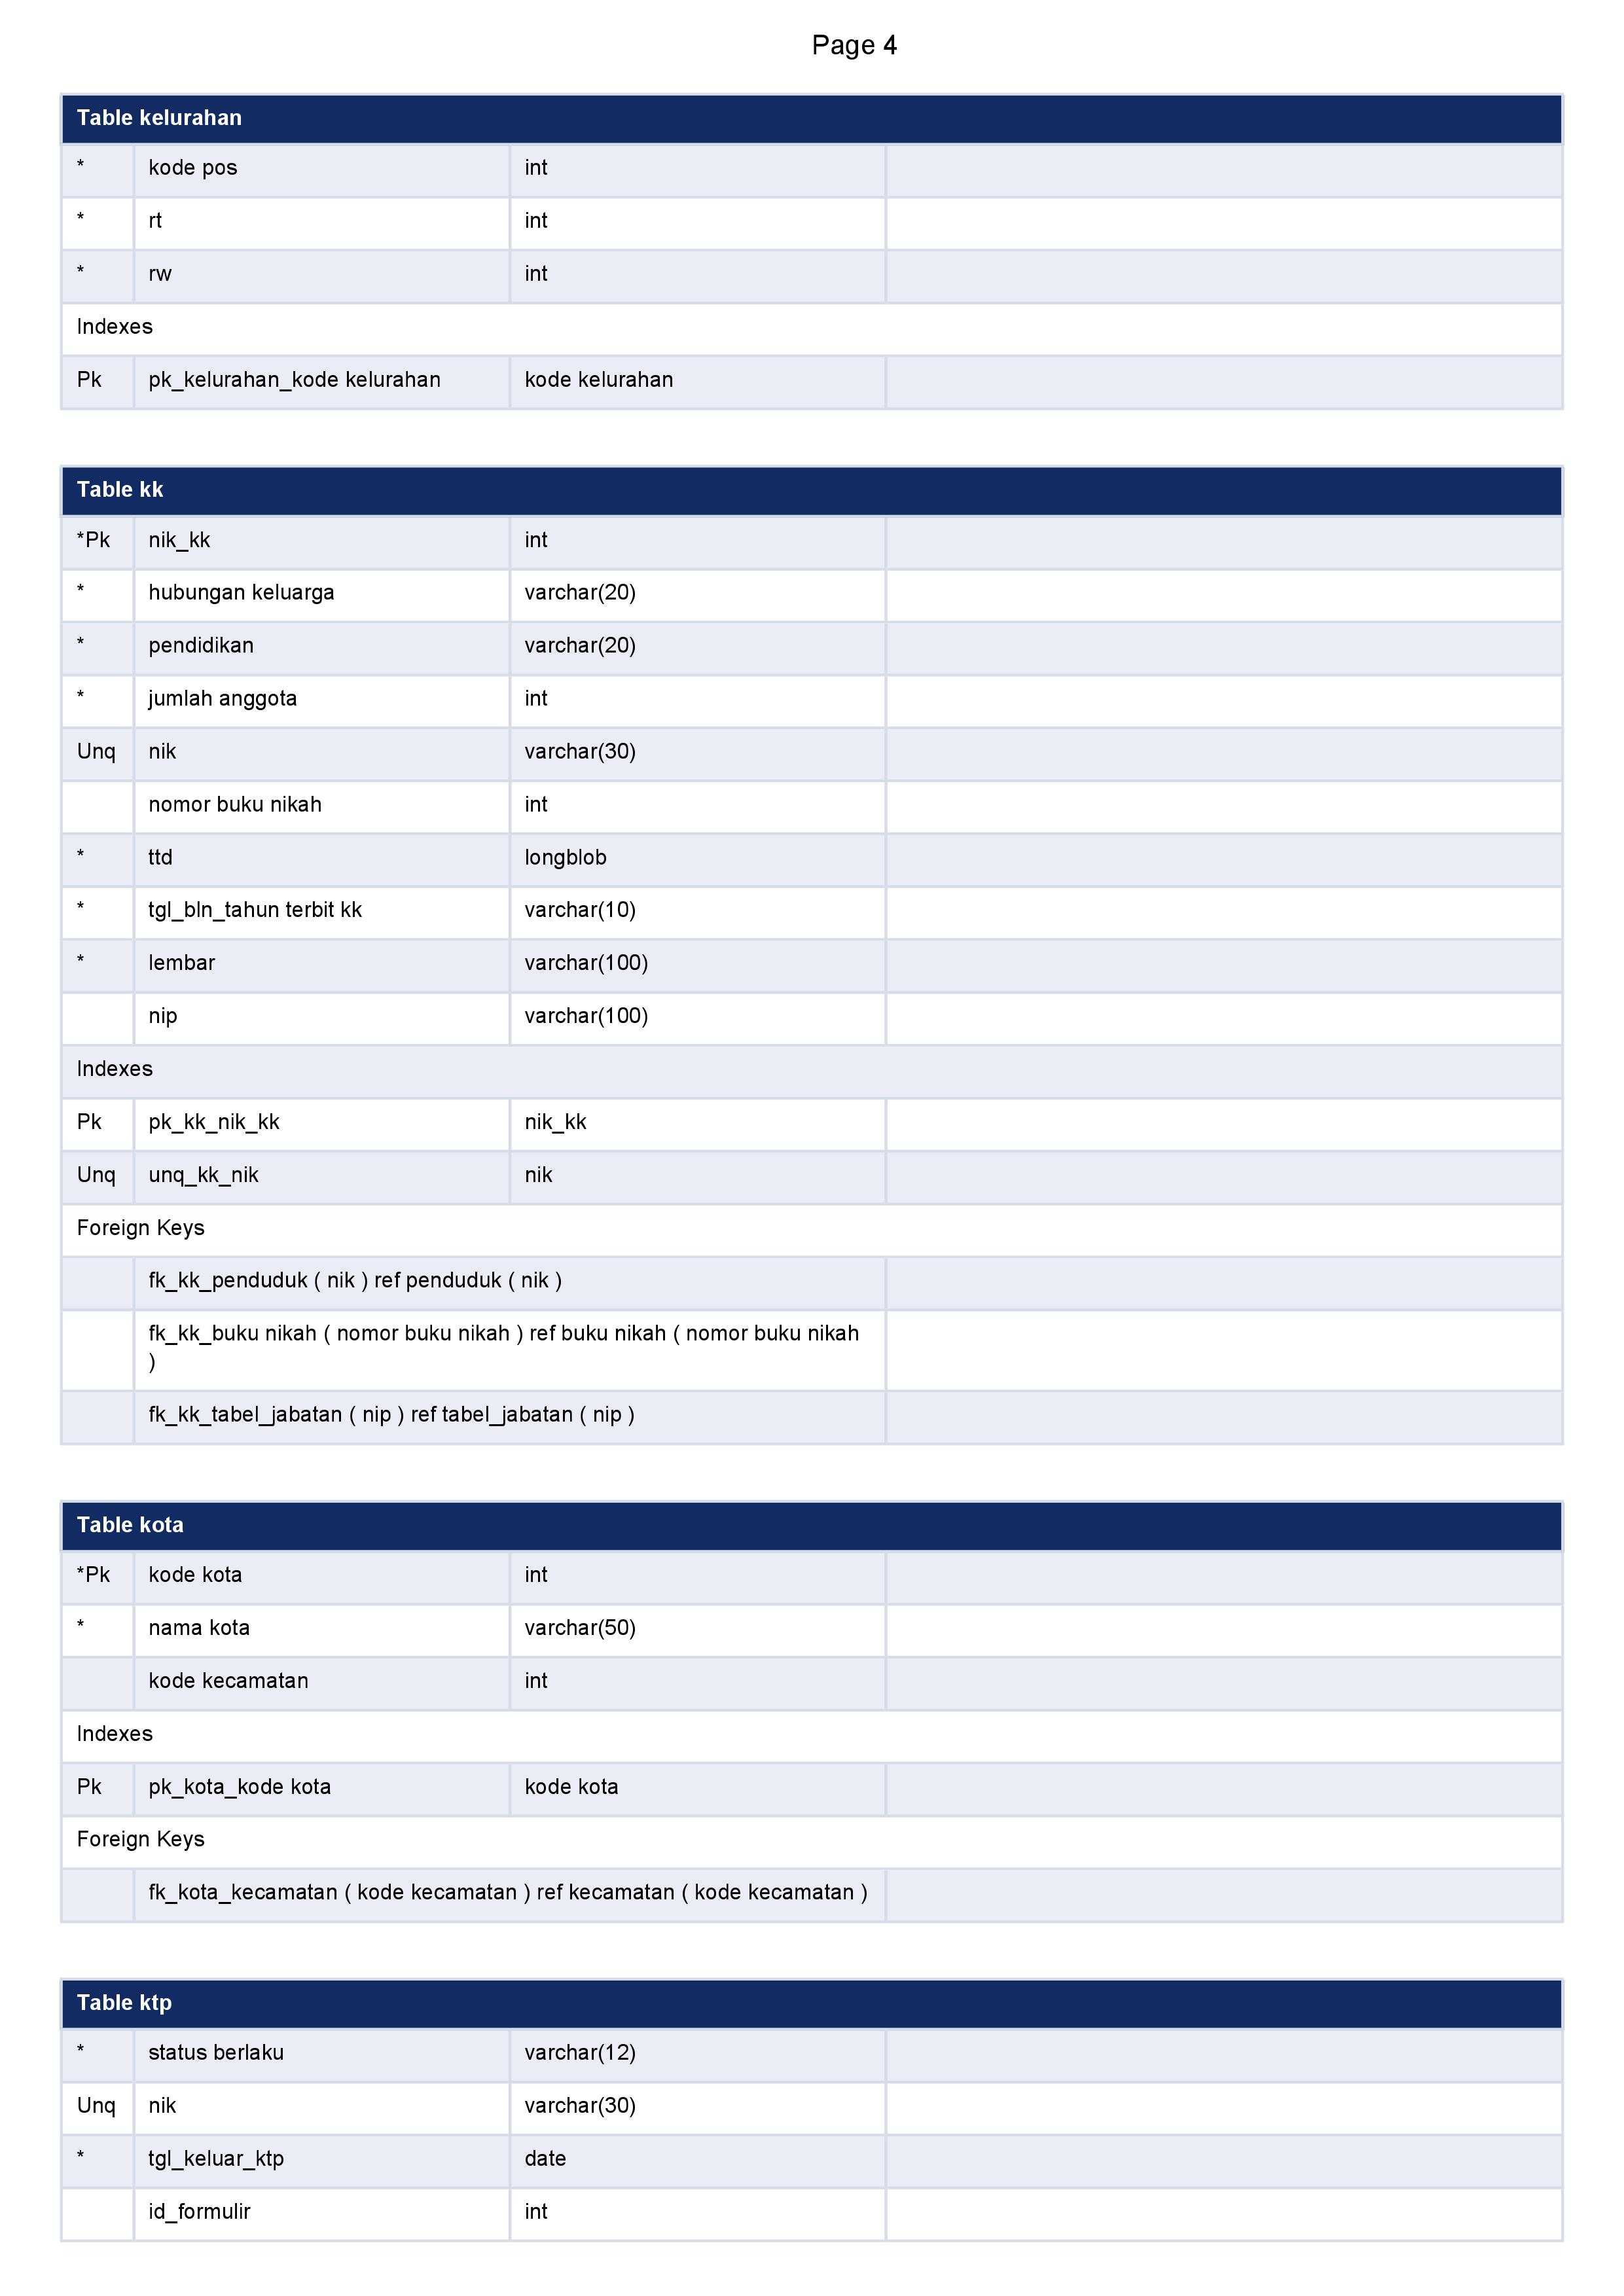
\includegraphics[width=12cm]{figures/0005.jpg}
	\caption{Relasi 3}
\end{figure}
\begin{figure}[H]
	\centering
	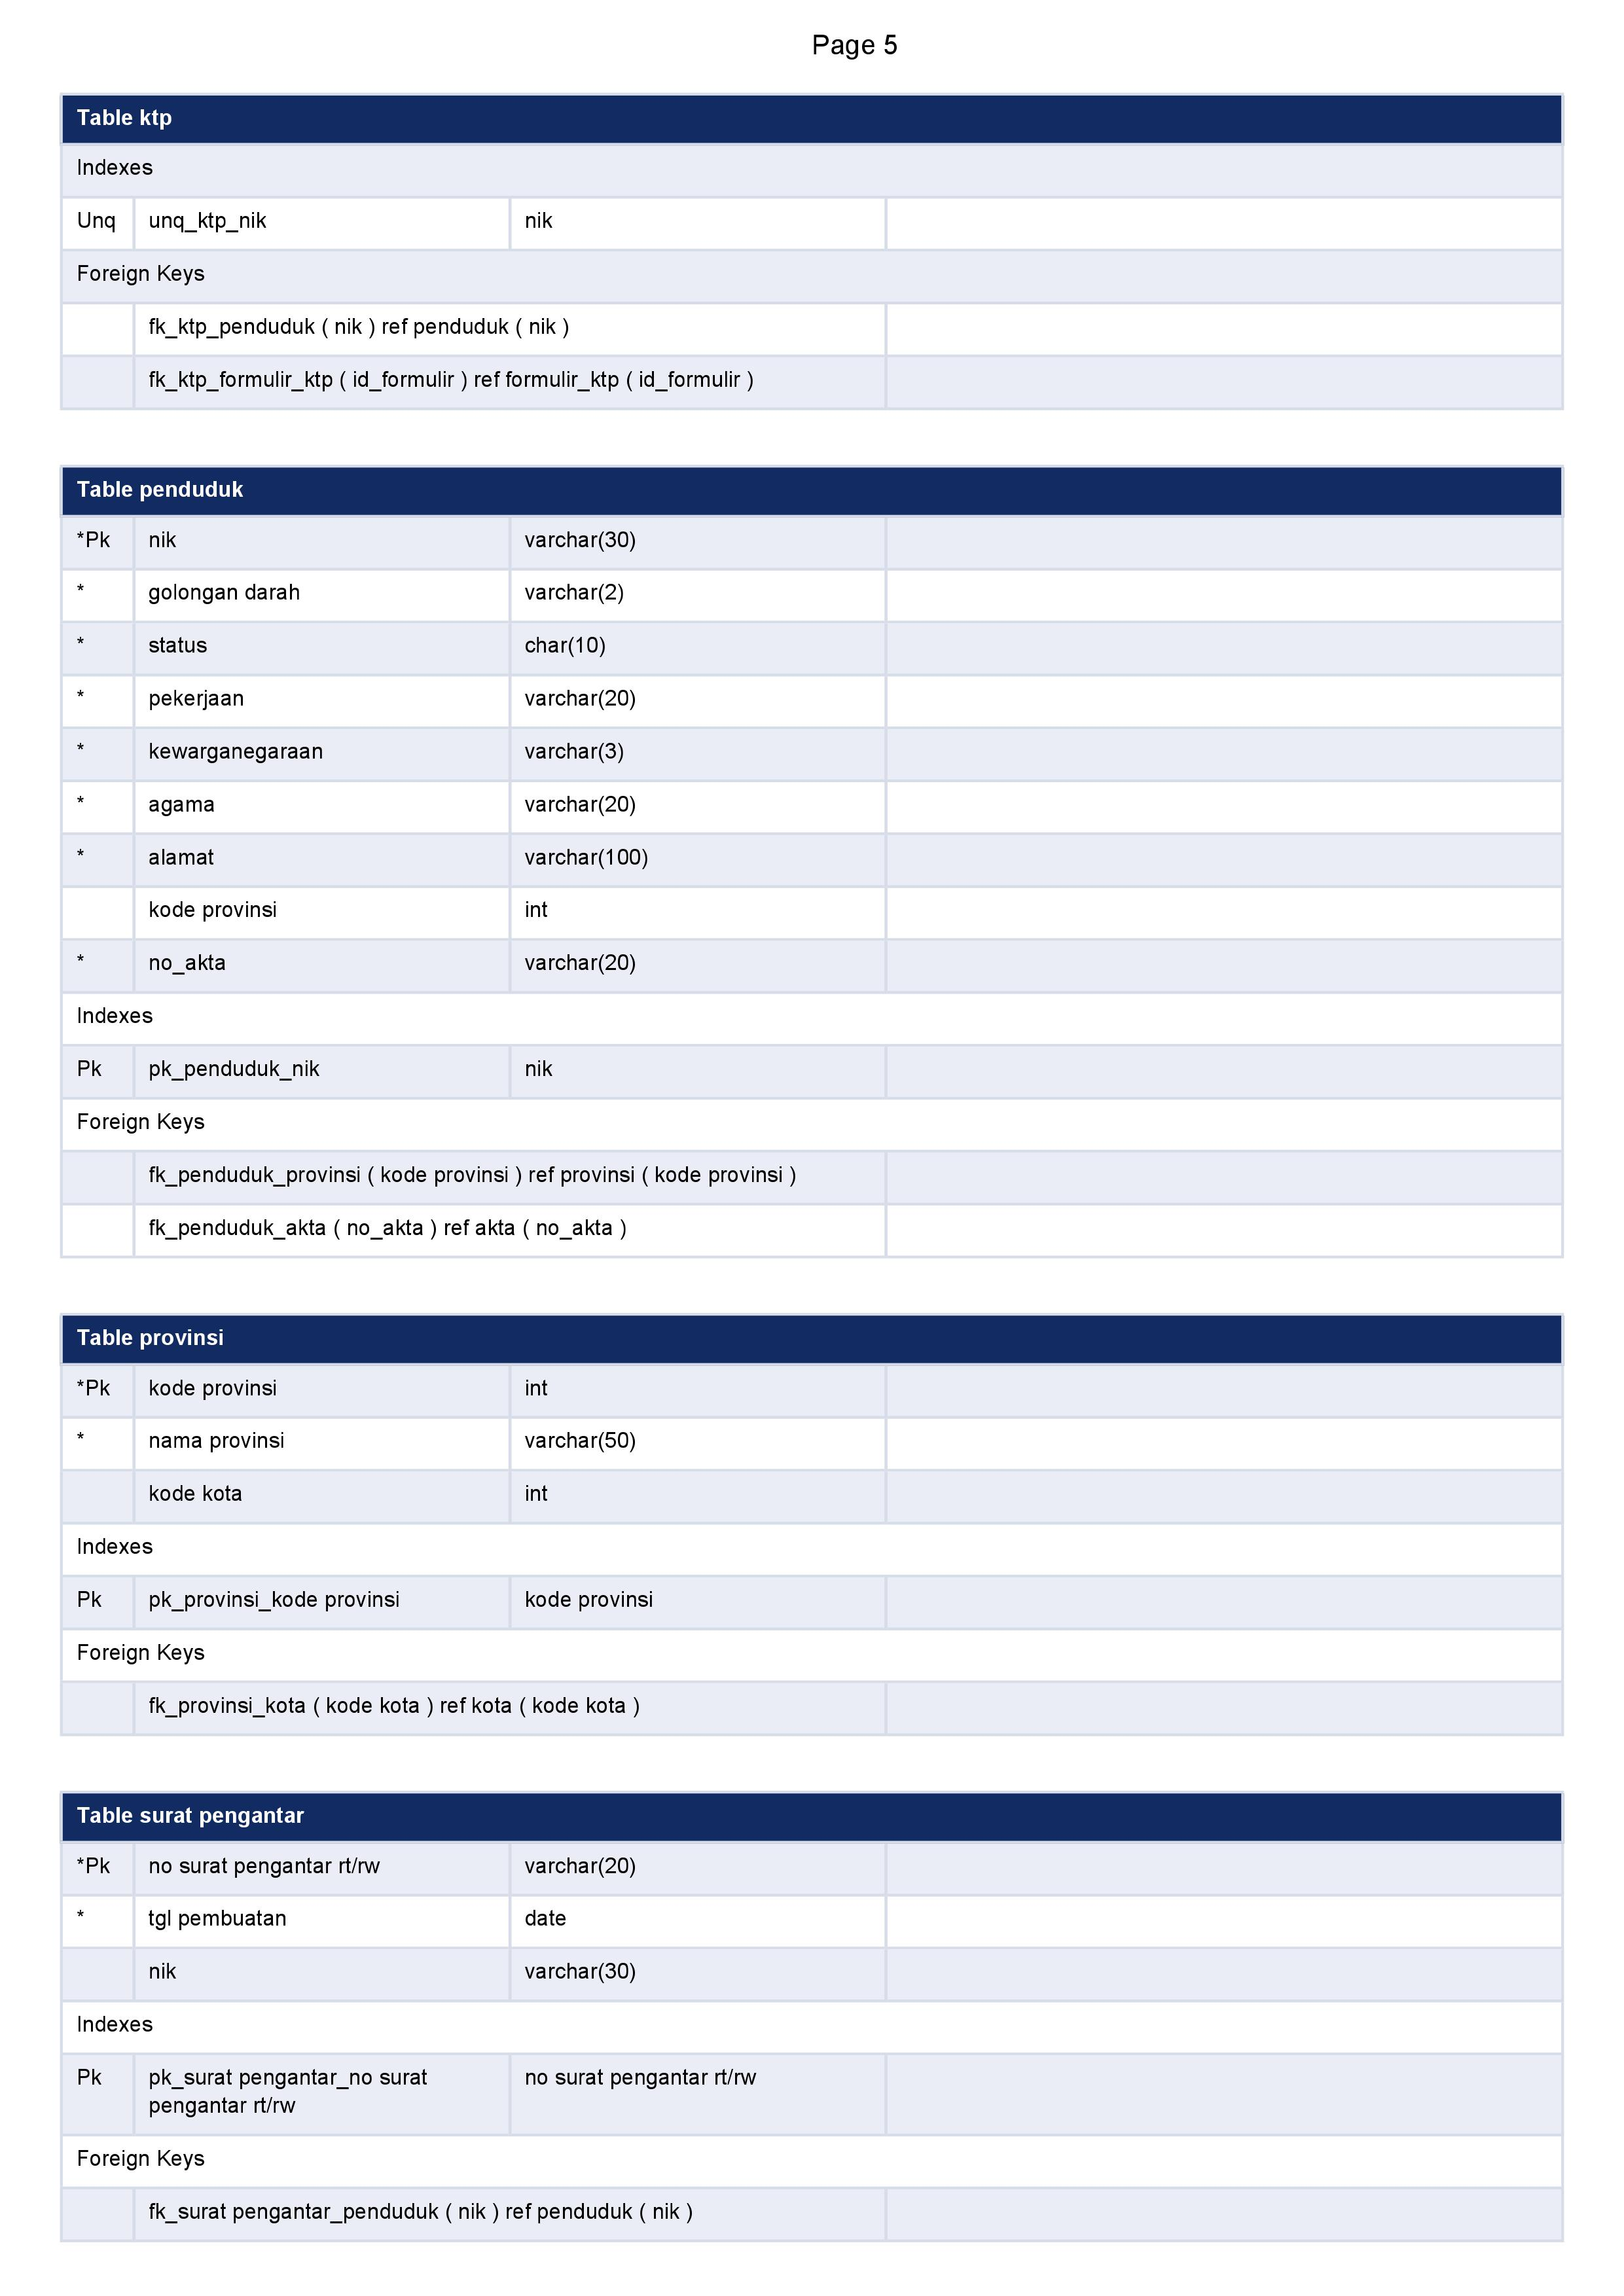
\includegraphics[width=12cm]{figures/0006.jpg}
	\caption{Relasi 4}
\end{figure}
\begin{figure}[H]
	\centering
	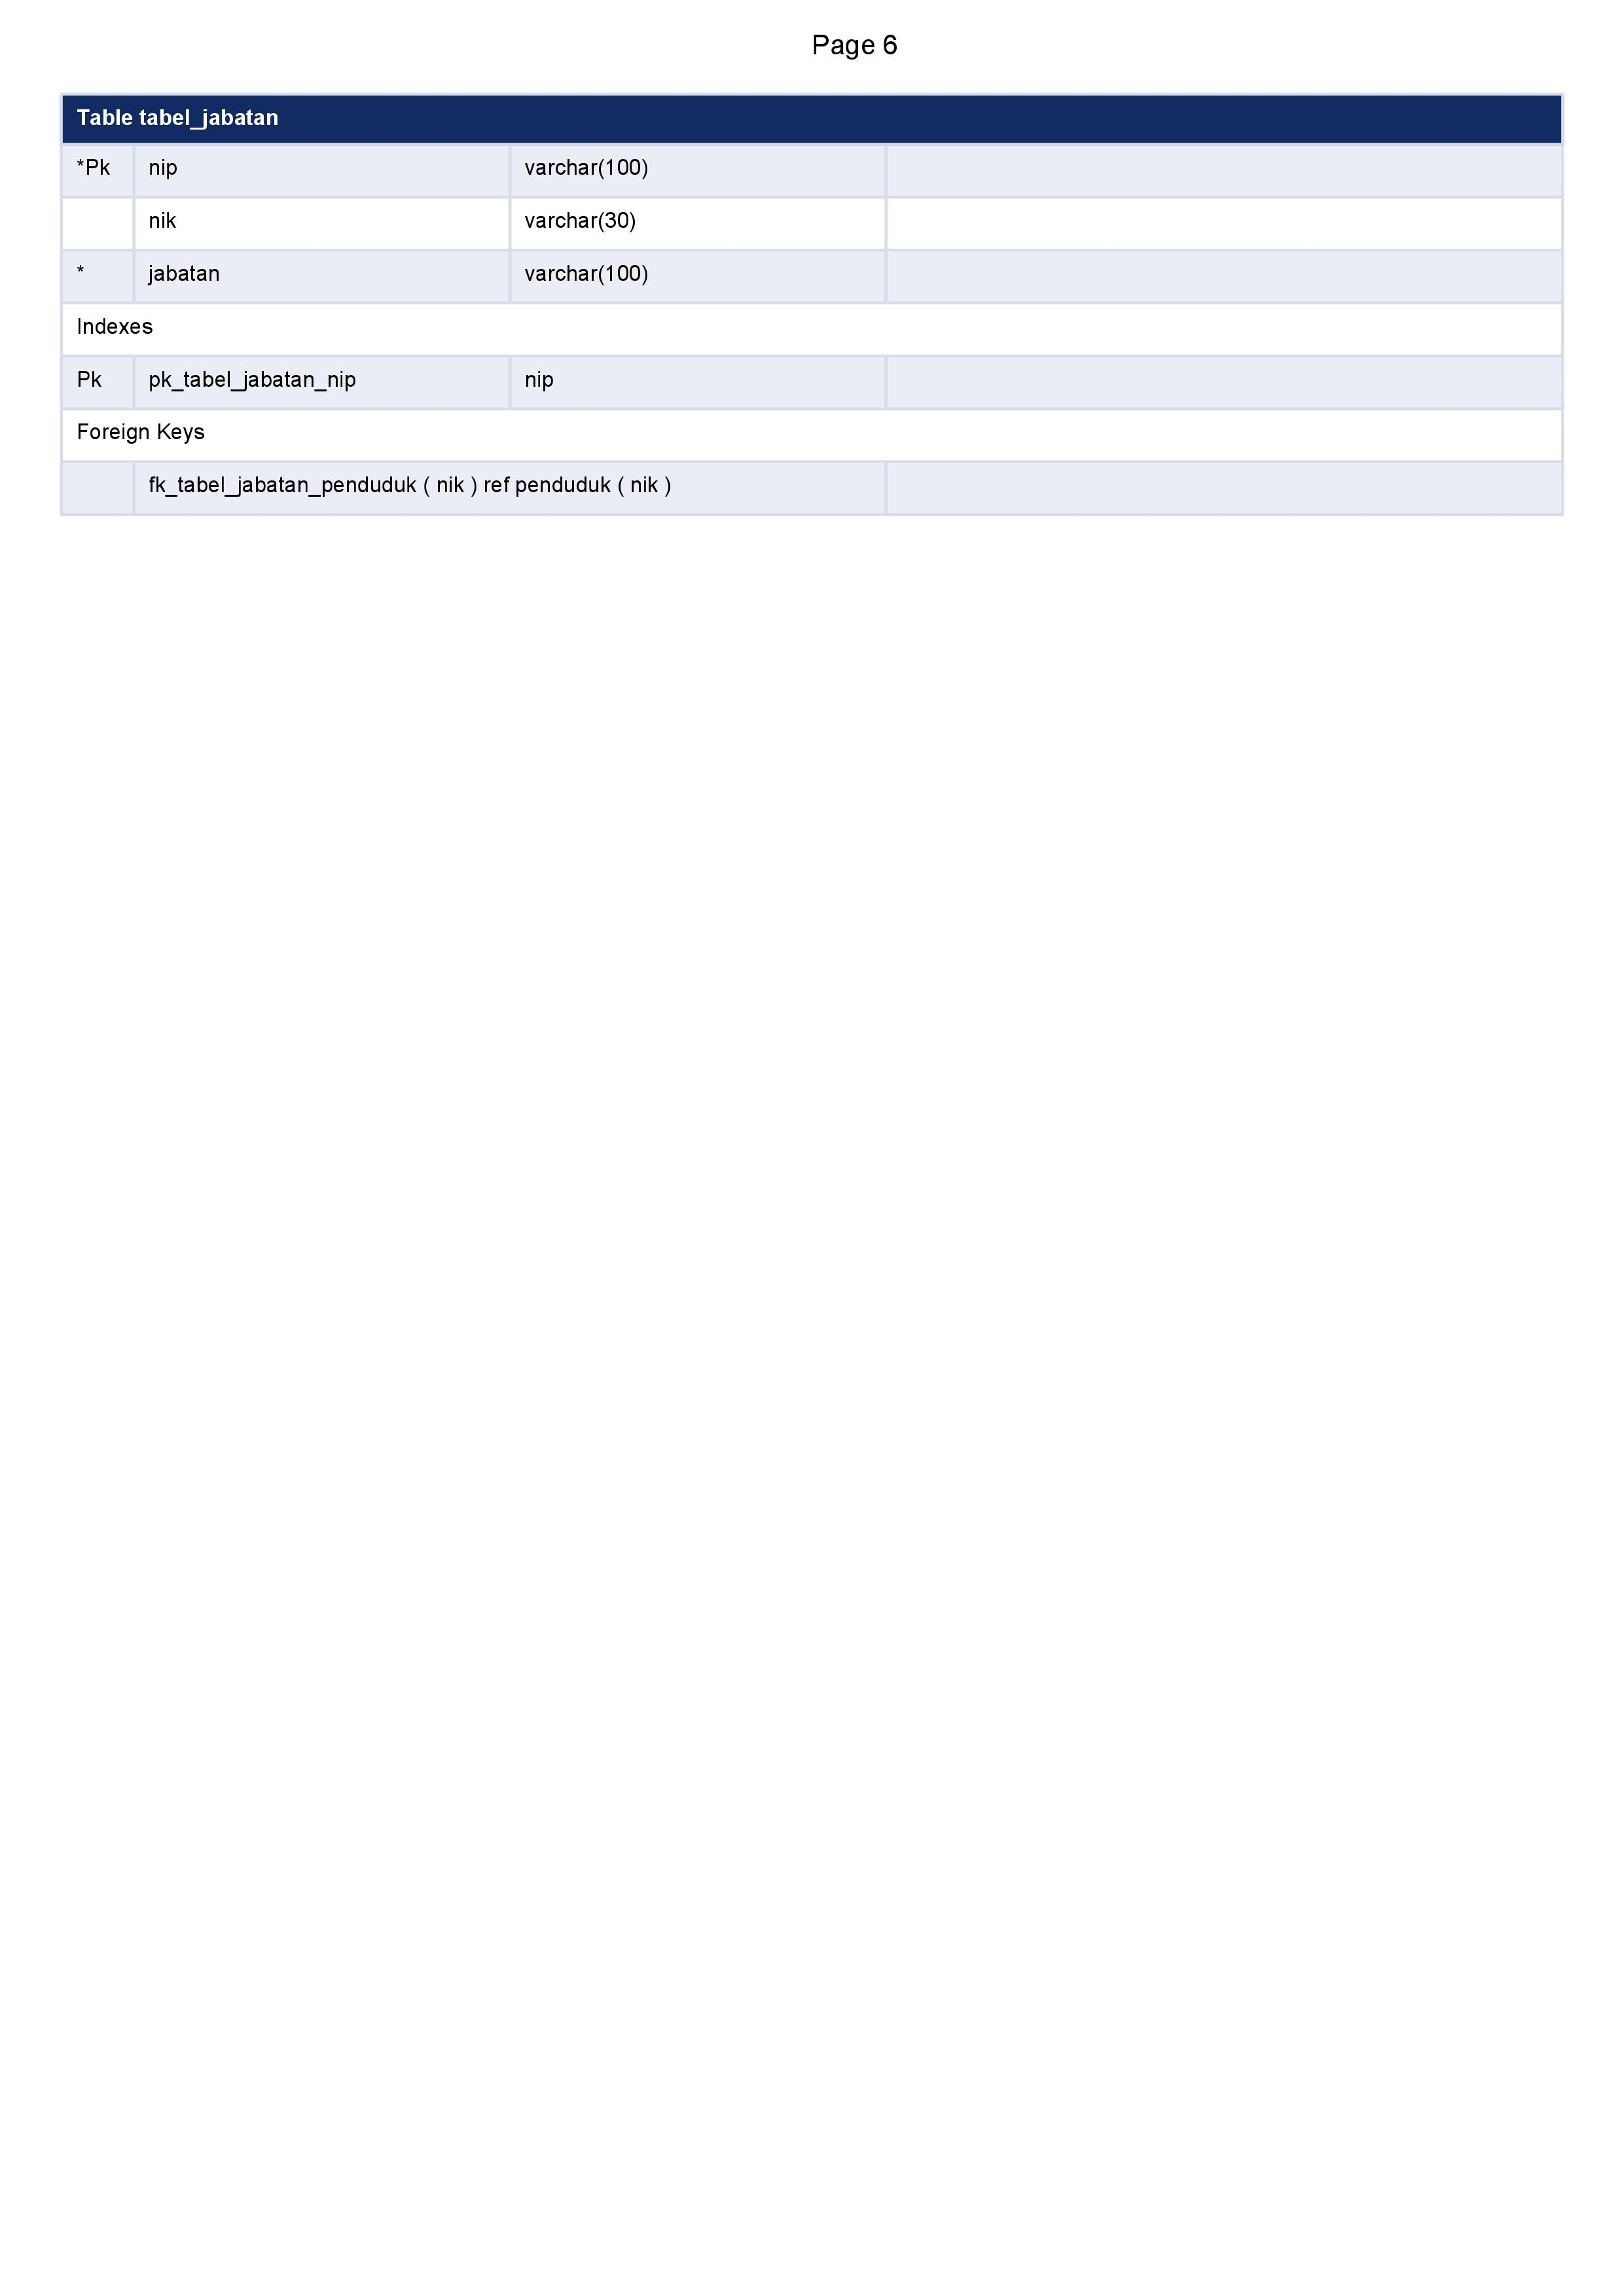
\includegraphics[width=15cm]{figures/0007.jpg}
	\caption{Relasi 5}
\end{figure}

\begin{table}
\centering
Relasi kardinalitas untuk tabel pembuatan e-KTP baru yaitu sebagai berikut :\\ [3ex]
		\begin{tabular}{|c|c|c|}
			\hline
			\textbf{Tabel}&\textbf{Kardinalitas}&\textbf{Tabel}\\
			\hline
			t.kk  & one-to-many  & t.penduduk  \\
			\hline
			t.penduduk  & one-to-one  & t.ktp  \\
			\hline
			t.formulirktp  & one-to-one  & t.ktp  \\
			\hline
			t.formulirkk  & one-to-one  & t.kk  \\
			\hline
			t.kelurahan  & many-to-one  & t.kecamatan  \\
			\hline
			t.kecamatan  & many-to-one  & t.kota  \\
			\hline
			t.kota  & many-to-one  & t.provinsi  \\
			\hline
			t.provinsi  & one-to-many  & t.formulirkk  \\
			\hline
			t.provinsi  & one-to-many  & t.formulirktp  \\
			\hline
			t.surat pengantar  & one-to-one  & t.formulirkk  \\
			\hline
			t.surat pengantar  & one-to-one  & t.formulirktp  \\
			\hline
			t.kk  & one-to-many  & t.formulirktp  \\
			\hline
			t.surat pengantar  & one-to-one  & t.penduduk  \\
			\hline
			t.penduduk  & one-to-one  & t.akta  \\
			\hline
			t.penduduk  & one-to-one  & t.jabatan  \\
			\hline
			t.penduduk  & one-to-one  & t.buku nikah  \\
			\hline
			t.jabatan  & one-to-many  & t.kk  \\
			\hline
			t.jabatan  & one-to-many  & t.akta  \\
			\hline
			t.buku nikah  & one-to-one  & t.kk  \\
			\hline
		\end{tabular}
\end{table}